\chapter{Introduction}
\section{A little motivation}

The desire to infer precise and accurate stellar ages is motivated by a range
of scientific drivers, but the one that most sparks my personal interest is
the implications for understanding the evolution of exoplanetary systems.
Despite the rapidly accelerating interest in exoplanet population studies
\citep[e.g.][]{petigura, dressing, foreman-mackey, burke}, we still know very
little about how planetary systems {\it evolve}.
This is because stellar ages are difficult to infer.

Planetary system architectures are not static in time: chaotic gravitational
interactions can fling planets into interstellar space, and plunge them into
the surface of their star.
If they cross orbits they can even collide and break apart or become excited
them to highly eccentric and inclined orbits.
Simulations of planetary systems often show that planet losses are most common
in the few millions of years immediately after formation and continue at a
gradually decreasing rate \citep[e.g.][]{zhou, smith, funk, Pu2015}.
Planet-planet scattering on extended timescales may result in a decrease in
exoplanet frequency with stellar host age in the enormous sample of over five
thousand exoplanets discovered to date {\it if} their ages can be sufficiently
constrained \citep{veras}.

Studying the exoplanet population as a function of age will unveil the
processes behind planet formation and dynamical evolution---two extremely
active areas of research.
By evaluating planet occurrence rates over a range of stellar ages it may be
possible to examine the dependence of overall occurrence on age and constrain
the rate of exoplanet loss.
Once the loss-rate is known we can extrapolate back in time to reveal what
zero-age planetary systems look like and possibly even to constrain the
primordial number of planets per star.

Stellar ages also provide a window into the {\it architectural}\/evolution of
planetary systems.
The exoplanet population shows a mysterious feature: half of all transiting
exoplanet systems have just one transiting planet and the other half have
multiple \citep[e.g.][]{lissauer, johansen, ballard}.
Additionally, the single planet systems, or `singles', are more often
misaligned with the spin-axis of their host star and have more eccentric
orbits than multiple planet systems, `multis' \citep[e.g.][]{morton, winn}.
This phenomenon is known as the `\Kepler\ dichotomy', and its origin is
a point of hot dispute: do two modes of formation create the distinct system
architecture?
\citet{Pu2015} propose an elegant solution: the singles are descended from the
multis, i.e.\ they are the remains of once ordered planetary systems, ripped
apart by chaotic gravitational interactions.
If this is the case, the singles may, on average, be older than the multis.
Most compact \Kepler\ multis are so tightly packed that they hover near the
stability limit \citep{fang}.
As the lifetime of a planetary system increases, so does its disruption
probability, therefore tightly-packed multis have shorter projected lifetimes
than loosely-packed systems.
By comparing the ages of tightly packed multis with the ages of loosely-packed
multis and the ages of singles it may be possible to reveal the dynamical
origins of the three groups.

Determining the detectability of trends in the ages of \Kepler\ systems is
challenging as the outcomes of simulations depend strongly on input
assumptions and different studies therefore produce different predictions
\citep[see figure 3 of][]{Pu2015}.
However, based on the \citet{smith} simulations of systems with three
Earth-mass planets, \citet{veras} demonstrate that a decrease in planet
occurrence rate will be detectable for K dwarf hosts, even if stellar age
uncertainties are as large as 5 Gyr, and for G dwarfs with age uncertainties of
3.5 Gyr.
Most systems do not consist of equal-mass planets, however their study
demonstrates that an age trend lies well within the realms of detectability.
Age precision will vary on a star-by-star basis, most likely ranging from
0.5-5 Gyr, however I expect to infer ages with uncertainties of $\sim$1 Gyr
for the majority of planet hosts and, thanks to the size of the \Kepler\
planet candidate sample, this will be more than sufficient to reveal trends in
the data.

This is just one of the tantalising scientific discoveries looming on the
horizon, if only we could improve our methods for inferring precise stellar
ages.
As I explain in this thesis, my research has advanced our understanding of the
stellar age-rotation, or `gyrochronology' relations \citep{angus}, which has
contributed to our ability as a community to infer stellar ages.
This research may ultimately lead to a discovery of variation in the
architecture and frequency of exoplanets as a function of host star age.

% Earlier this year I used \Kepler\ asteroseismic field stars to calibrate
% the gyrochronology relations at late ages, revealing a surprising result: the
% old targets rotated more rapidly than expected \citep{angus}.
% This finding provoked the response of \citet{vansaders} who attribute this
% behaviour to an evolving magnetic dynamo.
% Their result is important as it informs us over which range of stellar ages
% the gyrochronology method delivers precise results.
% Gyrochronology performs best for stars that are Solar-mass or below and/or
% those that are younger than the Sun.
% These criteria are met by most of the \Kepler\ stars: the age distribution
% peaks at around 2 Gyr and the mass distribution is centered on Solar-mass
% \citep{walk, mcquillan2014}.
% For many of these stars gyrochronology can yield stellar ages with 20\%
% precision \citep{epstein} and as demostrated by \citet{veras},
% a time-resolution of 20\% is more than sufficient to detect variations in the
% exoplanet occurrence rate over time.

\section{Kepler}

The \kepler\ spacecraft plays a starring role in this thesis, so I shall
introduce it now.
Launched in 2009, \kepler\ was designed to survey over a hundred-thousand
stars, searching for extrasolar planets.
Its ultimate goal was to answer the question "how common are Earth-like
planets in our galaxy?".
To date \kepler\ has discovered more than 5700 planet candidates and over 1000
confirmed planets.
These numbers are still growing at a breath-taking rate and planets are likely
to continue being discovered data well after the \kepler\ funding has dried
up, thanks both to the enormity of the data set and the continual improvement
of planet search methods.
\kepler\ produced high precision\footnote{Precision ranging from a few hundred
parts per million for bright (< 13th magnitude) targets to tens of thousands
of ppm for faint (> 17th magnitude) targets.} broad-band (peaking between V
and R bands) light curves for around 150,000 stars.
The majority of these stars were observed in long-cadence mode (once every
half-hour), and a few hundred in short cadence mode (once every minute),
continually for around four years.
Since it was necessary for \kepler\ to point at one field continually, it is
in a heliocentric orbit so that the Earth doesn't get in the way.
The \kepler\ field is centred at $\mathrm{RA} = 19\mathrm{h} 22\mathrm{m}
40\mathrm{s}$, $\mathrm{Dec} = +44^\circ30' 00'$, in the Cygnus region along
the Orion arm of the galaxy.
This field was chosen to be neither over nor under crowded, far enough out of
the ecliptic that the Sun never shines onto the detector and contamination
from Solar system objects is reduced.
\kepler\ has a limited amount of on-board storage and must point towards the
Earth to down-link data every month.
These pointings break the time series.
Other gaps appear at three month (quarter) intervals.
The spacecraft rotates every quarter to keep its Solar panels pointed at the
Sun.
The stars shift to new CCD modules every time this happens, eventually
returning to the same module after one year.
Both the down-link pointings and quarter rotations produce short gaps in the
light curves and can also produce short-term temperature changes to the CCD
which can effect the sensitivity of the detector.
Temperature changes increase the gain of the CCD chip: more electrons are
excited when the CCD is warmer so the flux appears to increase.
So despite the unprecedented precision of \kepler\ lightcurves, they are not
uninterrupted and contain systematic features.
Understanding the systematics in \kepler\ data is necessary for {\it all} of
\kepler's science goals and is a key part of this thesis.
This point is covered further in \textsection \ref{sec:detrending}.

Unfortunately, that key question---"how common are Earth-like planets?"---may
never be answered by \kepler \citep[or at least not very precisely, several
inferences have been performed by extrapolation, \eg][]{Foreman-Mackey2014,
Petigura2012, Burke2015}.
Although \kepler launched with four functioning gyroscopic reaction wheels,
one broke shortly thereafter.
This was not a mission-ender since the spacecraft only needed three to
maintain its precise pointing: one for pitch, one for roll and one for yaw.
Unfortunately however a second, this time mission-critical reaction wheel
broke in 2013.
Without all three reaction wheels, precise pointing of the spacecraft was
impossible to maintain in its current orientation.
The extreme precision of \kepler\ comes from its extreme pointing position.
With stars held fixed in place, moving by less than a pixel over a quarter,
% FIXME: how much?
even without knowing the exact Point Spread Function (PSF) and Pixel Response
Function (PRF), it is possible to perform precise relative photometry.
With it's pointing stability compromised, the community were asked for input
for a repurposed \kepler\ mission \citep[some examples here][]{Hogg2013,
Aigrain2013}.

\kepler\ was re-purposed as the \ktwo\ mission in 2014.
With just two reaction wheels controlling pitch and yaw, its third rotation
axis had to be stabilised.
This was achieved by balancing the spacecraft against Solar pressure, using
its symmetric solar-panelled back.
The spacecraft sits in an unstable equilibrium, drifting slowly about its roll
axis, its new orientation reducing large forces from the Solar wind
\citep{Howell2013}.
The spacecraft's thrusters are used to correct the slow drift.
Although the precision is not what it once was: stars drift across several
pixels before the thrusters correct the motion, it is still good enough to
perform plenty of science.
In order to keep its back to the Sun, \kepler\ can only point at fields in the
ecliptic plane.
This means that new stellar populations can be explored: from different
galactic regions, the bulge, thin and thick discs and halo, to open and
globular clusters.
Crucially, from the point of view of stellar astronomy, \kepler's new fields
incorporate several open clusters.
Open clusters are wonderful labs for stellar astronomy as they are coeval
populations of stars made from the same material.
They are controlled environments in which we can study the observational
properties of stars as a function of their mass.
Figure \ref{fig:current_fields} shows the current fields being observed by the
spacecraft and figure \ref{fig:future_fields} shows the future fields being
proposed.

\begin{figure}[p]
\begin{center}
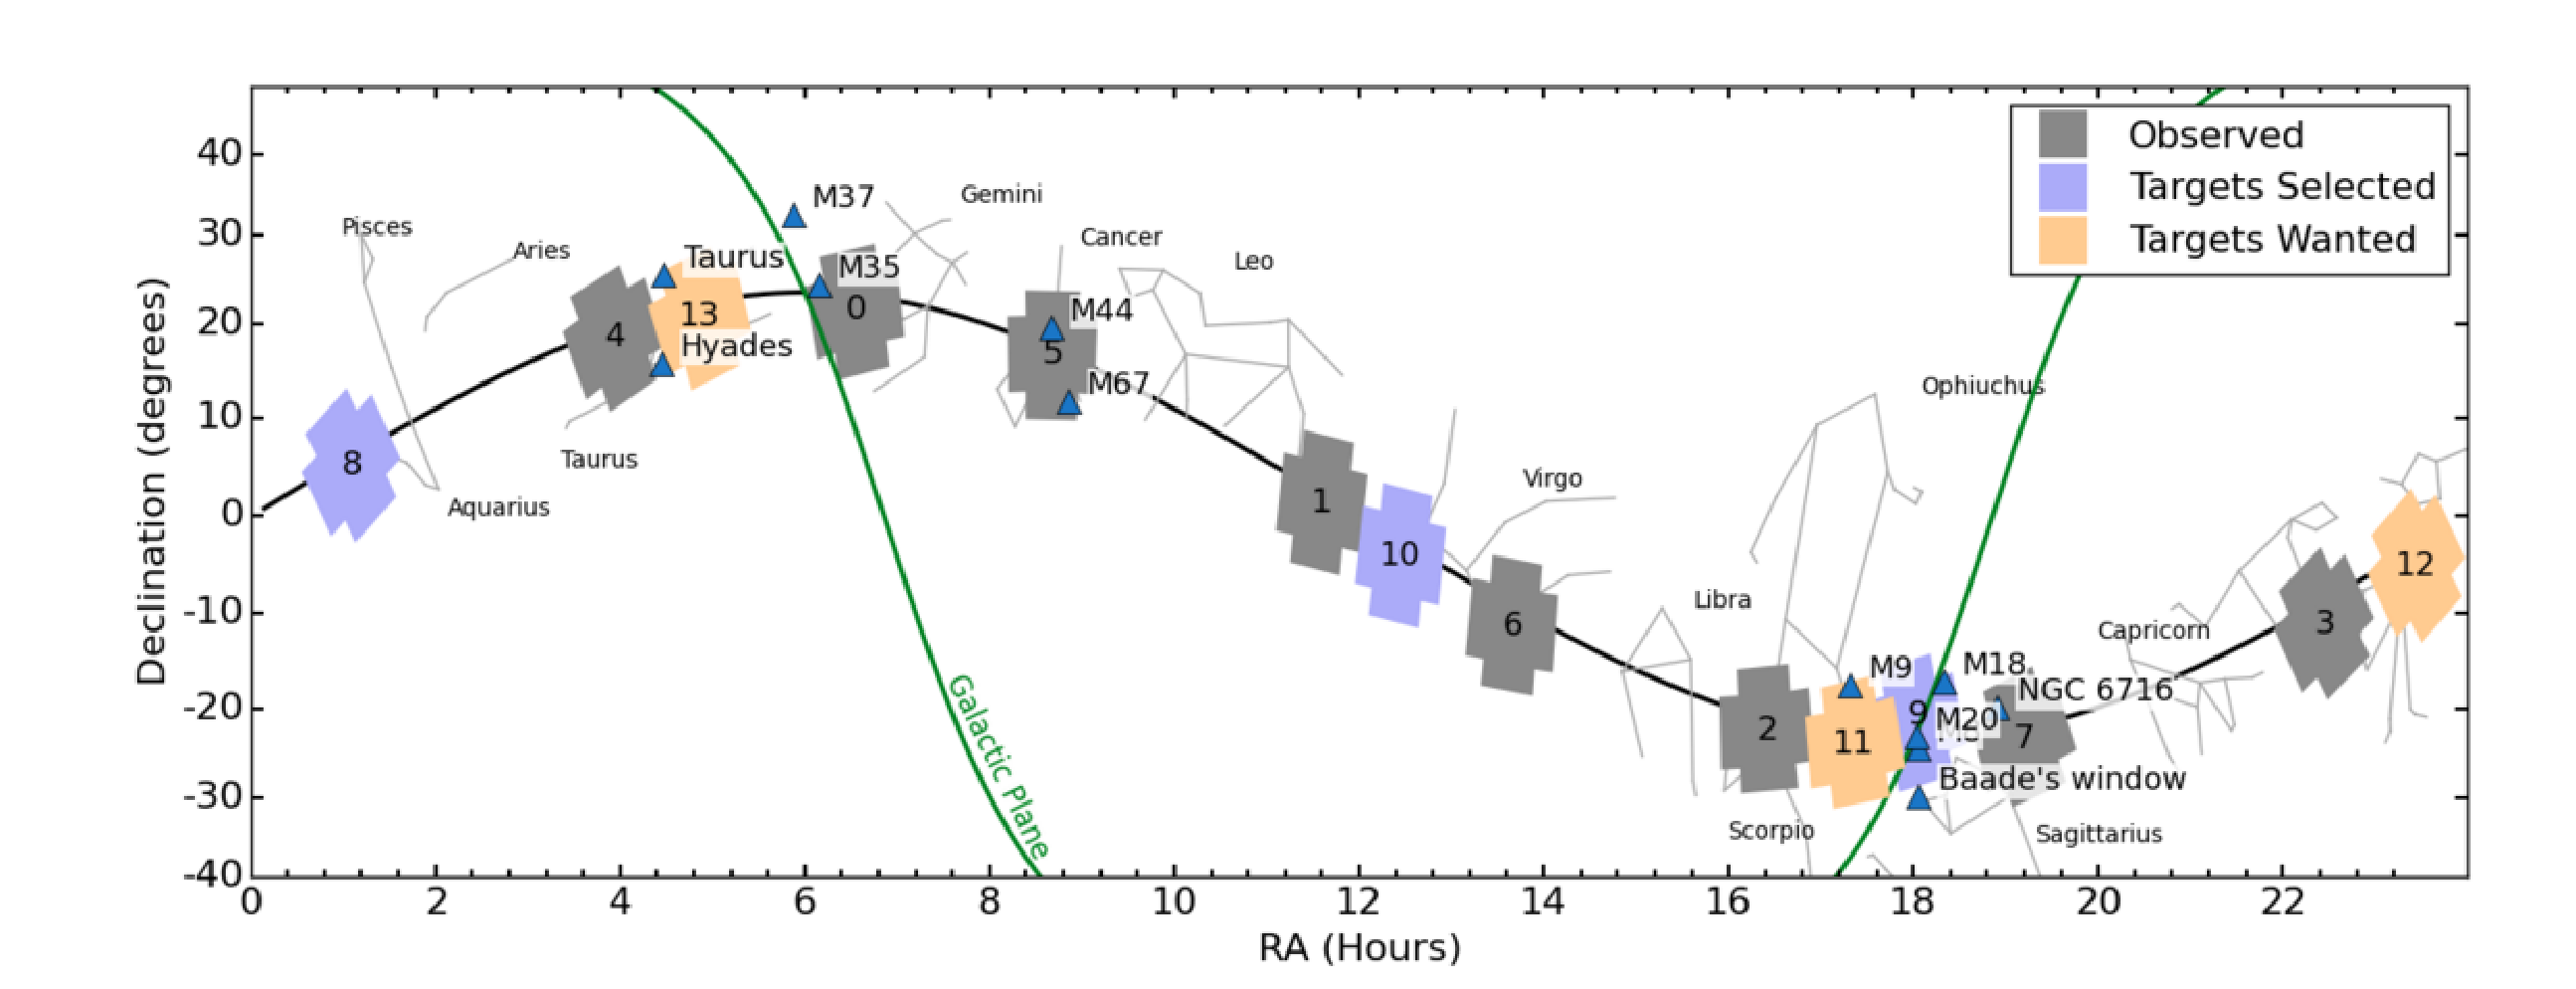
\includegraphics[width=6in, clip=true]{figures/Current_K2_fields.pdf}
\caption{\ktwo's fields. Fields 1-9 have already been observed and field 9 is
being observed at the time this thesis is handed in. Targets have been fixed
for purple fields and proposals are currently being solicited for yellow
fields.}
\label{fig:current_fields}
\end{center}
\end{figure}

\begin{figure}[p]
\begin{center}
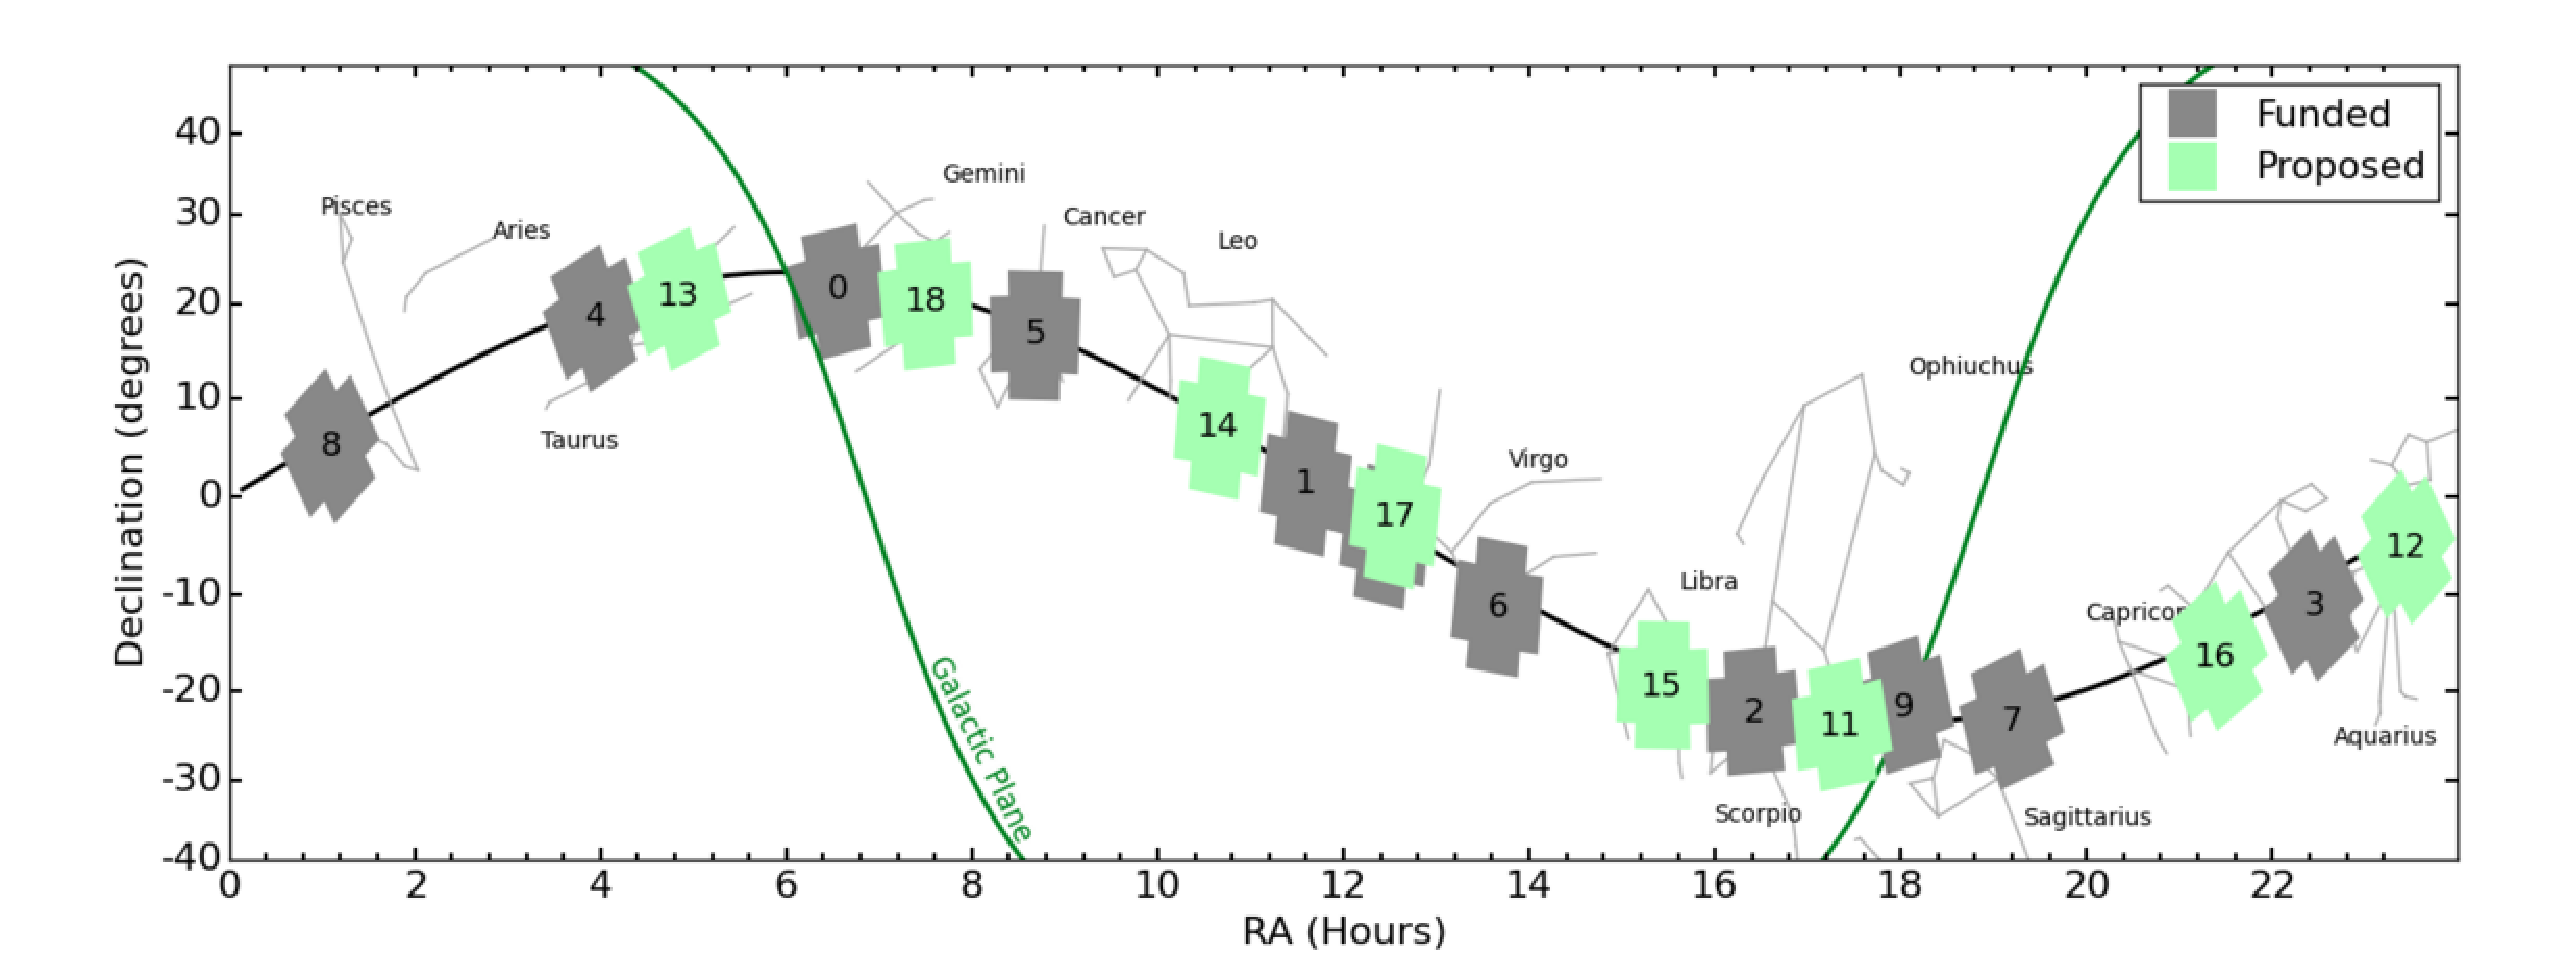
\includegraphics[width=6in, clip=true]{figures/Future_K2_fields.pdf}
\caption{\ktwo's current and future fields. These green fields are those
proposed if an extended \ktwo\ mission is funded.}
\label{fig:future_fields}
\end{center}
\end{figure}

Not only is the spacecraft continuing its search for exoplanets \citep[and has
already discovered many, \eg][]{Vanderburg2015, Crossfield2015,
Foreman-Mackey2015, Montet2015, Becker2015, Vanderburg2016}, it will
provide time series of white dwarfs, active galactic nuclei, red giants, red
dwarfs, binary stars and other interesting astronomical objects.
Of course, with the reduced pointing position comes a new challenge for
those astronomers willing to tote their data pick-axes to get at the science
gold-mine.
Systematic features in \ktwo\ light curves range from negliable for the
brightest targets to dominant for the faintest.
It is therefore necessary to do some digging to get at the good stuff.
This subject is covered in \textsection{sec:detrending}

\section{Stellar dating methods}

The hydrogen-burning era of a star's life is extremely stable.
This fact is unfortunate from a stellar chronologist's point of view as
without an observable property that is a strong function of age, stellar age
precision will always be limited.
This is the stumbling-block for stellar age inference: age precision is
restricted by the fundamental evolutionary time-scale of stars.
Despite this limitation however, there is still plenty of room for progress to
be made in understanding the evolution of the observable properties from both
empirical and theoretical standpoints, and in the precision with which we can
measure these properties.

Isochronal ages are notoriously difficult to infer because stars vary little
in brightness or temperature during their hydrogen-burning lifetimes.
Fitting stellar evolution models to these two observables usually produces age
estimates with uncertainties in the order of 50-150\%.
However, because cool stars spin down predictably over their main sequence
lifetime due to magnetic braking, their ages depend, to first order, only on
their masses and current rotation periods \citep[e.g.][]{skumanich, kawaler,
barnes}.
Photometric measurements of these two parameters can therefore be used to
infer an age.
The concept of `gyrochronology'---inferring an age from a rotation period---
developed after observations of stars in clusters revealed a trend for
decreasing rotation period with time.
This method has never held so much promise as it does now, with a new glut of
stellar rotation periods available from a new generation of spacecraft
designed for high precision, high cadence photometry.
The main science goal for these missions are searching for exoplanets, but the
exoplanet gold-rush has lead to a new understanding of stars and what we can
learn about them from the way their brightness varies alone.
The desire to develop a method of dating stars using only photometry is an
understandable one with the current availability of such large photometric
data sets.
However, as with any phenomenological investigation, inferences about the data
can only be made with models.
These models can be physical or empirical but whatever the origin of their
design, they must be calibrated using observations.
No age model can exist in isolation from observations---our understanding of
stars just isn't good enough.
So when a new dating method is developed, its efficacy relies on the existence
(and precision) of previous dating methods.
It is therefore important to understand the currently available dating
methods, their advantages and their limitations.
I describe the main methods used today in the following section.

\subsection{Isochrone fitting}

As stars burn hydrogen they become hotter and more luminous, slowly moving
towards the top right of the Hertzprung-Russel Diagram (HRD), or
Colour-Magnitude Diagram (CMD).
If you can infer a star's absolute magnitude and effective temperature or
measure its colour and you have an idea of its composition and evolutionary
stage, you can place it on an HRD or CMD and infer its age.
In practice it usually is not possible to input magnitude, temperature,
metallicity and \logg into a model, crank the handle and pull out an age.
The computation that goes into those models are expensive, so the variation in
luminosity and temperature over time has been modelled by several teams of
astronomers who produce sets of model grids.
In order to infer an age from the observations therefore, it is necessary to
interpolate between the nearest grid lines and the actual position of your
star on an HRD or CMD.
The Dartmouth \citep{dotter}, Yonsei-Yale \citep{spada} models are two of the
most commonly used sets of models.

An obvious limitation of this method is that the composition of the star in
question will affect its placement on a HR/CMD: a more metal-rich star will
appear cooler and redder than a more metal-poor one with the same mass and
age.
% FIXME: why?
It is often difficult or impossible to obtain precise metallicities, helium
abundances and alpha-element fractions (all needed for precise isochrone
placement) as these measurements come from expensive, high-precision
spectroscopy.
% FIXME: how are these things actually extracted from spectra?
However, for an ensemble of coeval stars with identical compositions this
process becomes much easier: not only are there more opportunities to measure
stellar compositions, providing a $\sqrt N$ reduction in measurement
uncertainty, a group stars with the same age and composition but different
masses will reveal the shape of the best-fitting isochrone on the CMD\@.
This reduces the need for knowing composition precisely in the first place.
For these reasons, many open stellar clusters have very precise ages.

% For example Pleiades (0.55 Gyr), Hyades (0.625 Gyr), Praesepe (0.588 Gyr), and
% Coma Berenices (0.5 Gyr).
% Download isochrones and estimate the ages of some KOIs.

\subsection{Asteroseismology}

\kepler\ prime's success story is not limited to exoplanets: stellar astronomy
itself has been advanced and arguably the second most important branch of
\kepler\ prime's legacy is asteroseismology.

\kepler\ operates in two observing modes: long and short cadence
\citep[][]{smith2012, stumpe2012}.
Long cadence observations are taken every approximately 30 minutes, with ...
minute integration times and short cadence observations are taken every minute
with ... second integration times.
The frequencies that are accessible to \kepler\ are limited by two things: the
duration of observations and the time sampling.
The duration of observations, e.g. the length of the \kepler\ mission sets the
minimum resolvable frequency.


Asteroseismology is a powerful dating method with the potential to yield
extremely precise stellar ages.
However, the era of asteroseismology has only just arrived and this fledgling
field is still only applicable to a small number of extremely bright stars
observed by precise photometric space-missions.

Oscillations in the Sun are caused by turbulent convection near the surface.
The movement of ionized gas stochastically excites the Sun's spherical
oscillation modes.
An analogy to this process is that of a bell in a room filled with air.
Air particles colliding with the surface of the bell cause it to vibrate at
all of its spherical harmonic frequencies.
There is no coherent driving force, rather the stochastic collisions of air
particles induce a continual ringing.
Similarly, the Sun is continually oscillating at a range of discrete
frequencies; those that correspond to its spherical harmonics.
A power spectrum of the Sun, taken from \citet{brown} is shown in figure
~\ref{solar_spectrum}.
The comb-like, evenly spaced peaks in this power spectrum show Solar p-mode
oscillations.
The peak amplitudes are modulated by a Gaussian envelope.
The mean of that Gaussian, $\nu_{max}$ corresponds to a frequency of around
3000 \uHz, a period of around five minutes.

\begin{figure}[p]
\begin{center}
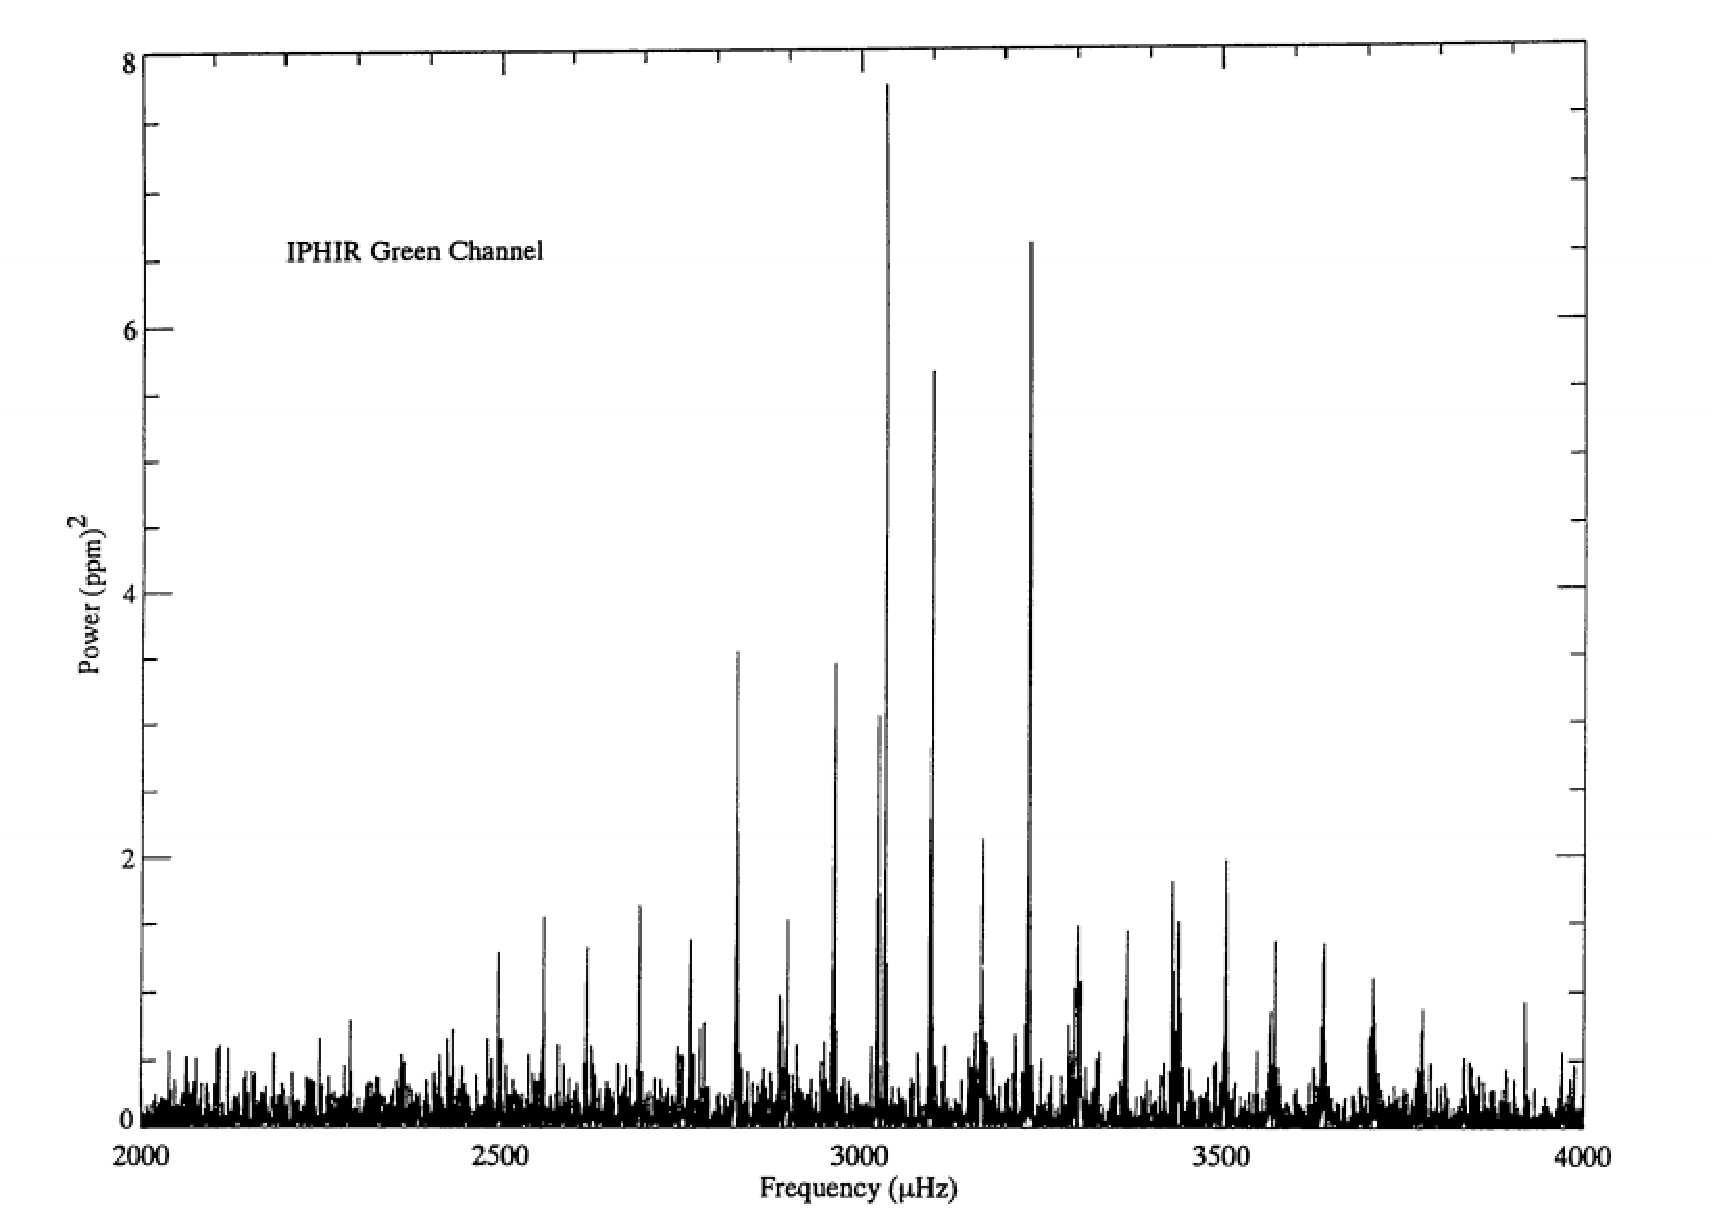
\includegraphics[width=6in, clip=true]{figures/solar_spectrum.pdf}
\caption{A power spectrum of one month of disk-integrated Solar photometry,
taken from \citet{toutain}. Solar p-modes are clearly visible in this figure.}
\label{fig:solar_spectrum}
\end{center}
\end{figure}

Many properties of the Sun have been measured using asteroseismic pulsations.
For example, the variation in radial pressure, the rate of differential
rotation, the depth and fraction of helium in its convective zone and even the
structure of active regions below the Solar surface.
The Sun is an exquisite example of a pulsating star, having tens of millions
of detectable modes and mode lifetimes that are several thousand times longer
than the periods of the oscillations.
Its proximity, which both provides enormous signal-to-noise and allows us to
resolve the surface, make it a paragon of seismology.

Three types of oscillations are detectable in the Sun: pressure, or p-modes,
surface, s-modes and gravity, g-modes.
Pressure provides the restoring force for p-mode oscillations, and these are
effectively sound waves.
Surface modes are, as the name suggests, waves on the surface of the star.
% Since it is only possible to detect s-mode waves if the stellar surface is
% resolvable, this type of wave has only been seen in our Sun.
G-modes are excited by buoyant gas in the radiative zone and the restoring
force is gravity, hence the name.
These waves rapidly evanesce in stellar convective zones and therefore
appear at very low amplitudes at the surface of Sun-like stars.
For the work in this thesis I am concerned only with p-mode observations, as
these waves reveal the internal structure of a star which varies as a function
of mass, radius and age.

The frequency of a p-mode wave is proportional to the sound-speed of the gas
along its path through the stellar interior.
Time-dependent spatial perturbations to a star's equilibrium state can be
written as a product of a term that depends on stellar radius and a spherical
harmonic (assuming that a star can be approximated as a sphere) as follows
\citep{brown},
\begin{equation}
    \xi_{nlm}(r, \theta, \phi, t) = \xi_{nl}(r)Y_l^m(\theta, \
    \phi)e^{-i\omega_{nlm}t}.
\end{equation}
$\xi$ is a spatial perturbation, associated with a mode, $r, \theta, \phi,
\omega$ and $t$ are the radial coordinate, colatitude, longitude angular
frequency\footnote{The convention in asteroseismology is to report circular
frequencies, $\nu_{nlm} = \omega_{nlm}/2$.} and time, respectively.
$n$ is the radial order, defined as the number of nodes between the star's
centre and surface and $l$ is the angular degree, the product of the stellar
radius and the total horizontal wavenumber of the mode.
For example, a star oscillating with an $l = 10$ mode will have a standing
wave with 10 nodes along a line around the equator.
Finally, $m$ is the azimuthal order; the projection of $l$ onto the horizontal
wavenumber of mode and must be less than or equal to $l$.
A star with an $m = 5$ mode will have a standing wave with 5 nodes along a
line connecting its poles.
The relation between $\omega$ and $n$ and $l$ is complicated and depends on the
structure of the star.
Oscillations with different values of $l$ penetrate to different depths in the
star.
$l = 0$ waves travel through the centre and waves with increasing $l$ skirt
the central region by a larger and larger distance.
For this reason, modes with different $l$ provide information about the sound
speed gradient in the stellar interior.
The `small frequency separation', $\delta_{n,l} = \nu_{n+1, l} - \nu_{n, l+2}$
is often used to parameterise the variation in frequency with stellar radius
via \citep{brown}
\begin{equation}
    \delta_{n,l} = \Delta\nu_0\frac{(l + 1)}{2\pi^2\nu_{nl}}\int_0^{R_\star}
    \frac{dc}{dr}\frac{dr}{r}.
\end{equation}
Since nuclear-burning material in the core changes its molecular weight as the
star evolves, the sound-speed gradient is time-dependent and the small
separation therefore contains information about the age of the star.

There is no simple harmonic relation between the frequencies of modes with
adjacent mode number \citep{brown}.
% check this!
However, in the limit where $n \gg l$, mode frequency can be approximated as
\begin{equation}
    \nu_{nl} = \Delta\nu_0\left(n + \frac{l}{2} + \epsilon \right) - \
    \frac{AL^2 - \eta}{(n + l/2 + \eta)},
\end{equation}
where parameters $\Delta\nu_0$, $A$, $\epsilon$ and $\eta$ depend on the
structure of the star and $L^2 = l(l+1)$.
$\Delta\nu_0$ is the `large frequency separation' which, together with the
peak frequency of the Gaussian envelope that modulates the amplitudes of the
oscillation modes, $\nu_{max}$, makes up the two fundamental asteroseismic
observables.
It is related to the sound travel time through the centre of the star:
\begin{equation}
\Delta\nu_0 = \left(2\int_0^{R_\star}\frac{dr}{c}\right)^{-1},
\end{equation}
where $c$ is the local sound speed and $R_\star$ is the stellar radius.
This travel time is related to the mean density of the star via,
\begin{equation}
\Delta\nu_0 \cong 135\left(\frac{M_\star}{R_\star^3}\right)^{1/2}\mu Hz,
\end{equation}
where $M_\star$ and $R_\star$ are the stellar mass and radius in Solar units
\citep{cox, brown}.

Today, p-modes have been detected in hundreds of Sun-like stars, however it
was not until the late 1990s that the first conclusive detection was made in
a star other than our Sun.
The reason for this is simply that p-mode perturbations are extremely
small---these changes are around 10 cms$^{-1}$ in velocity and 3$\mu$mag in
brightness for typical oscillation modes in the Sun \citep{brown2000}.
Asteroseismic pulsations are usually detected in two different ways: by
searching for the subtle change in luminosity caused by the temperature
fluctuations of the stellar surface, or by measuring the changing radial
velocity of the surface.
A Fourier transform of these time series will reveal the presence of
oscillation modes, allowing for the modelling of the star's interior
structure.
The earliest p-modes detections were made using radial velocity data
\citep{kjeldsen2001} for stars $\eta$ {\bf Boo} \citep{kjeldsen1995}, {\bf
Procyon} \citep{barban1999, martic1999}, $\zeta$ {\bf Herculis}
\citep{martic2001}, $\alpha$ {\bf Cen A} \citep{kjeldsen1999} and $\beta$ {\bf
Hyi} \citep{bedding2001}.
Today, we have the advantage of space-based missions \kepler\ and \corot whose
photometric precision provides sufficient signal-to-noise to detect
p-mode-induced luminosity variations.
These missions have provided fundamental parameters for hundreds of
oscillating giants, subgiants and Sun-like stars \citep[e.g.][]{michel2008,
bruntt2009, chaplin2014}.

% Extracting fundamental parameters from time series.
\subsection{Fundamental parameters from photometric time series}

In the previous section I describe the relations between stellar p-mode
oscillation frequencies and the physical parameters of a star.
In this section I will describe the application of asteroseismology: how
exactly does one infer fundamental stellar parameters from a light curve?
My thesis work focuses on \kepler\ data, so this discussion will be directly
related to \kepler\ data, but the same principles apply to other photometric
time series.

This branch of astronomy is still relatively young and, given the quantity of
up-and-coming photometric space missions, will continue to provide precise
stellar parameters for decades to come.
However, accurate and precise asteroseismic ages demand high-precision
photometry of bright (brighter than around 12th magnitude) stars.
Even with \kepler\ and \corot, this only amounts to around one hundred MS
stars.
It is therefore essential that alternative dating methods, which can be
applicable to a much larger sample of stars are developed.
Age-rotation relations, for example.

Asteroseismology is the way forward for fundamental stellar parameters.
It provides precise and accurate parameters, against which models for age,
mass and radius can be calibrated.

\subsection{Age-rotation relations}

Asteroseismology is revolutionising stellar astronomy and, perhaps, stellar
ages in particular (partly because the bar is so low to begin with).
However, it is not yet ready to  revolutionise fields involving stellar
populations because it is still a `boutique' method, applied to hand-picked,
bright, text-book Solar-like oscillators.
In order to produce a catalogue of stellar ages that is large enough to be
useful for studies of stellar populations, we need a method that can be
applied to thousands of stars \ie requires inexpensive observables, is not
computationally expensive and doesn't require human input (can be automated).
For this reason gyrochronology, the method of inferring an age from a rotation
period is an intriguing prospect as, if demonstrably accurate, fulfills all
the above criteria.
In what follows I describe the physics behind gyrochronology.

\citet{Skumanich1972} provided one of the first observational indications that
stellar rotation periods decay over time; they observed that rotation period,
lithium abundance and chromospheric activity decay was proportional to the
square-root of age.
In figure \ref{fig:skumanich}, equatorial rotational velocity vs time
(triangles) is plotted on the same axes as lithium abundance (crosses) and
Ca$^+$ emission (circles) for the Hyades and Pleiades clusters, as well as the
Sun.
The Sun is the far right point for each age indicator.
Only the equatorial velocities of the G stars in the two clusters are
indicated.
Ursa Major stars are included on the Ca$^+$ emission scale.
Lithium abundance and Ca$^+$ emission were previously known age indicators and
this work demonstrated the potential of rotation period as another.

\begin{figure}
\begin{center}
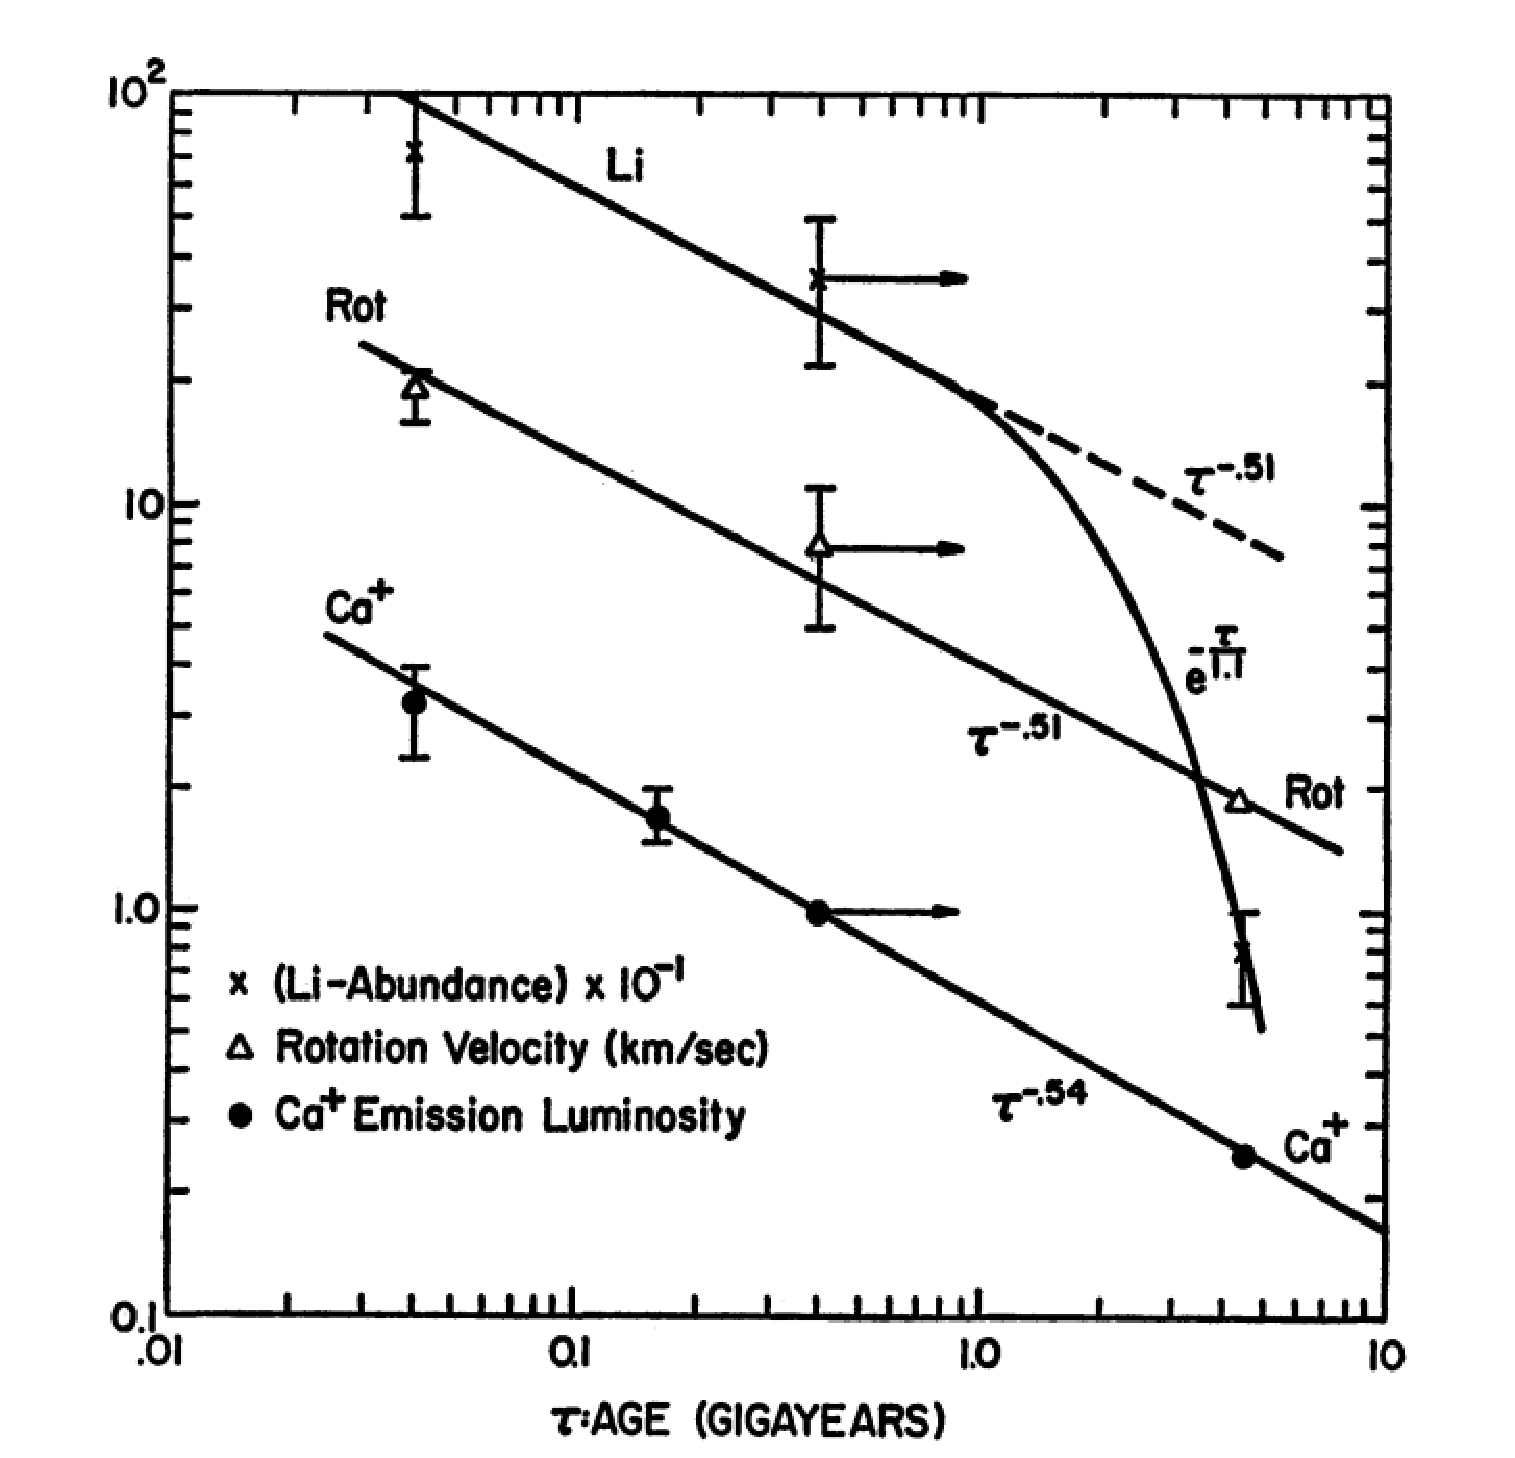
\includegraphics[width=4in, clip=true]{figures/skumanich.pdf}
\caption{Figure from \citet{skumanich1972}. Rotation periods for the G stars
in the Hyades and Pleiades and the Sun are plotted.}
\label{fig:skumanich}
\end{center}
\end{figure}

% The rotation periods of cluster stars were investigated in several studies
% \citep[\eg][]{Stauffer1987}.
% The physical mechanism behind the coupling of stellar winds to the magnetic
% dynamo was explored by \citet{Weber1967, Mestel1984}.
% This process was later applied to evolving stars by \citet{Kawaler1988}.
Today, we know that the angular momentum loss is caused by the magnetically
driven stellar wind \citep{Schatzman1962, Weber1967, Mestel1984}.
The stellar wind is made up of charged ions that stream away from the stellar
surface.
Each of these ions carries mass, charge and angular momentum as it travels
away from the star.
The star therefore loses mass, charge and angular momentum over its lifetime.
The angular momentum carried by these particles is lost from the system, not
necessarily at the surface, but at the point where they no longer rotate with
the star.
Stellar magnetic fields trap these particles, forcing them to rotate with the
same angular velocity as the surface out to the Alfv{\'e}n radius.
The Alfv{\'e}n radius is the point at which a particle experiences equal force
from the magnetic field and the pressure produced by surrounding particles.
Once they are beyond the Alfv{\'e}n radius, the particles' angular momentum is
lost from the star.
This dominant mechanism by which stars lose angular momentum during their
stint on the MS.
The stellar wind also carries mass away from the star, and the internal
structure of the star changes due to core hydrogen burning which both change
the star's moment of inertia, however these are secondary effects.

Stellar magnetic fields are generated in their convection zones.
The motion of turbulent plasma in the outer layers of intermediate-mass stars
acts like a dynamo, driving the production of magnetic fields.
% FIXME: how does rotation drive the dynamo?
Convective turbulence, combined with stellar rotation produces the large-scale
magnetic fields that lock the stellar wind to the star.
It is believed that rotation period influences magnetic field strength: more
rapid rotators have stronger magnetic fields.
The relation between angular momentum loss rate and the angular velocity of
rotation is a power-law, where the exponent depends on the magnetic field
geometry \citet{Mestel1984, Kawaler1988}.
Magnetic field strength controls the rate of angular momentum loss: a stronger
magnetic field leads to a larger Alfv{\'e}n radius which increases the angular
momentum loss per unit time.
% There is a saturation point however, angular momentum loss rate only increases
% with magnetic field strength up to a point \citet{Chaboyer1995, Sills2000}.
It is for this reason that the rate of angular momentum loss is not constant.
As a star loses angular momentum its rotation period decays and with it, its
magnetic field strength, so the rate of angular momentum loss decreases.
This process acts to force stellar rotation periods to converge.
% \citet{Reiners2012} showed that angular momentum evolution is a function of
Rapid rotators have a greater angular momentum loss rate than slower rotators.
Their rotation periods therefore decay more rapidly than slow rotators and,
after a few hundred million years low mass stars appear to rotate at a rate
that depends, to first order, only on their age and mass.
This convergence happens more quickly for early-type stars than late-type.
Whilst FGK stars may have converged by 500 million years, \citep{Radick1987,
Irwin2009} late M dwarfs may not converge within a Hubble time.

Since the magnetic dynamo is believed to be generated in the convective zone,
stars with a thin convective layer have a weaker magnetic field.
For this reason they lose angular momentum more slowly.
Angular momentum loss rate therefore varies as a function of stellar mass and
fully radiative stars do not spin down appreciably over their MS lifetime
\citet{Noyes1984_2}.
The rotational evolution of stars at the low-mass end, those that are fully
convective is still unknown.

\citet{Barnes2003} compiled rotation period measurements from members of
several young clusters and the Mt. Wilson stars.
% (CITATION)
When plotting stellar rotation periods against their B-V colours they noticed
that there were two morphological features of the data (see their figure 2).
For each cluster there was a sequence of stars falling neatly on the predicted
relation between rotation period and mass (called interface, or `I' stars),
but there were also a group of stars that were rotating rapidly (called
convective `C' stars).
These two sequences were most obvious in the younger clusters and less so in
the older.
\citet{Barnes2003} attributed this behaviour to an evolving magnetic dynamo,
produced by the still evolving internal structure of the young stars,
postulating that the I sequence is reduced for older stellar populations.
In this work I will only address stars that have already (in theory) already
transitioned from the C sequence to the I sequence as they are older than the
Hyades which is the last cluster to show this behaviour.
\citet{Irwin2009} compiled rotation period measurements for stars in open
clusters with masses $< 1.2 M_\odot$, shown in figure \ref{fig:irwin}.
The clusters shown here increase in age from the top left to the bottom right.
These data show the enormous spread in rotation periods for the youngest
clusters, contrasted with the extremely well-defined rotational sequence in
the Hyades (second panel from the bottom on the right).
The currently accepted view is that after the age of the Hyades, stellar
rotation periods lie on this converged sequence.
In what follows I will, for the most part, only discuss stars older than
around the age of the Hyades.

\begin{figure}[p]
\begin{center}
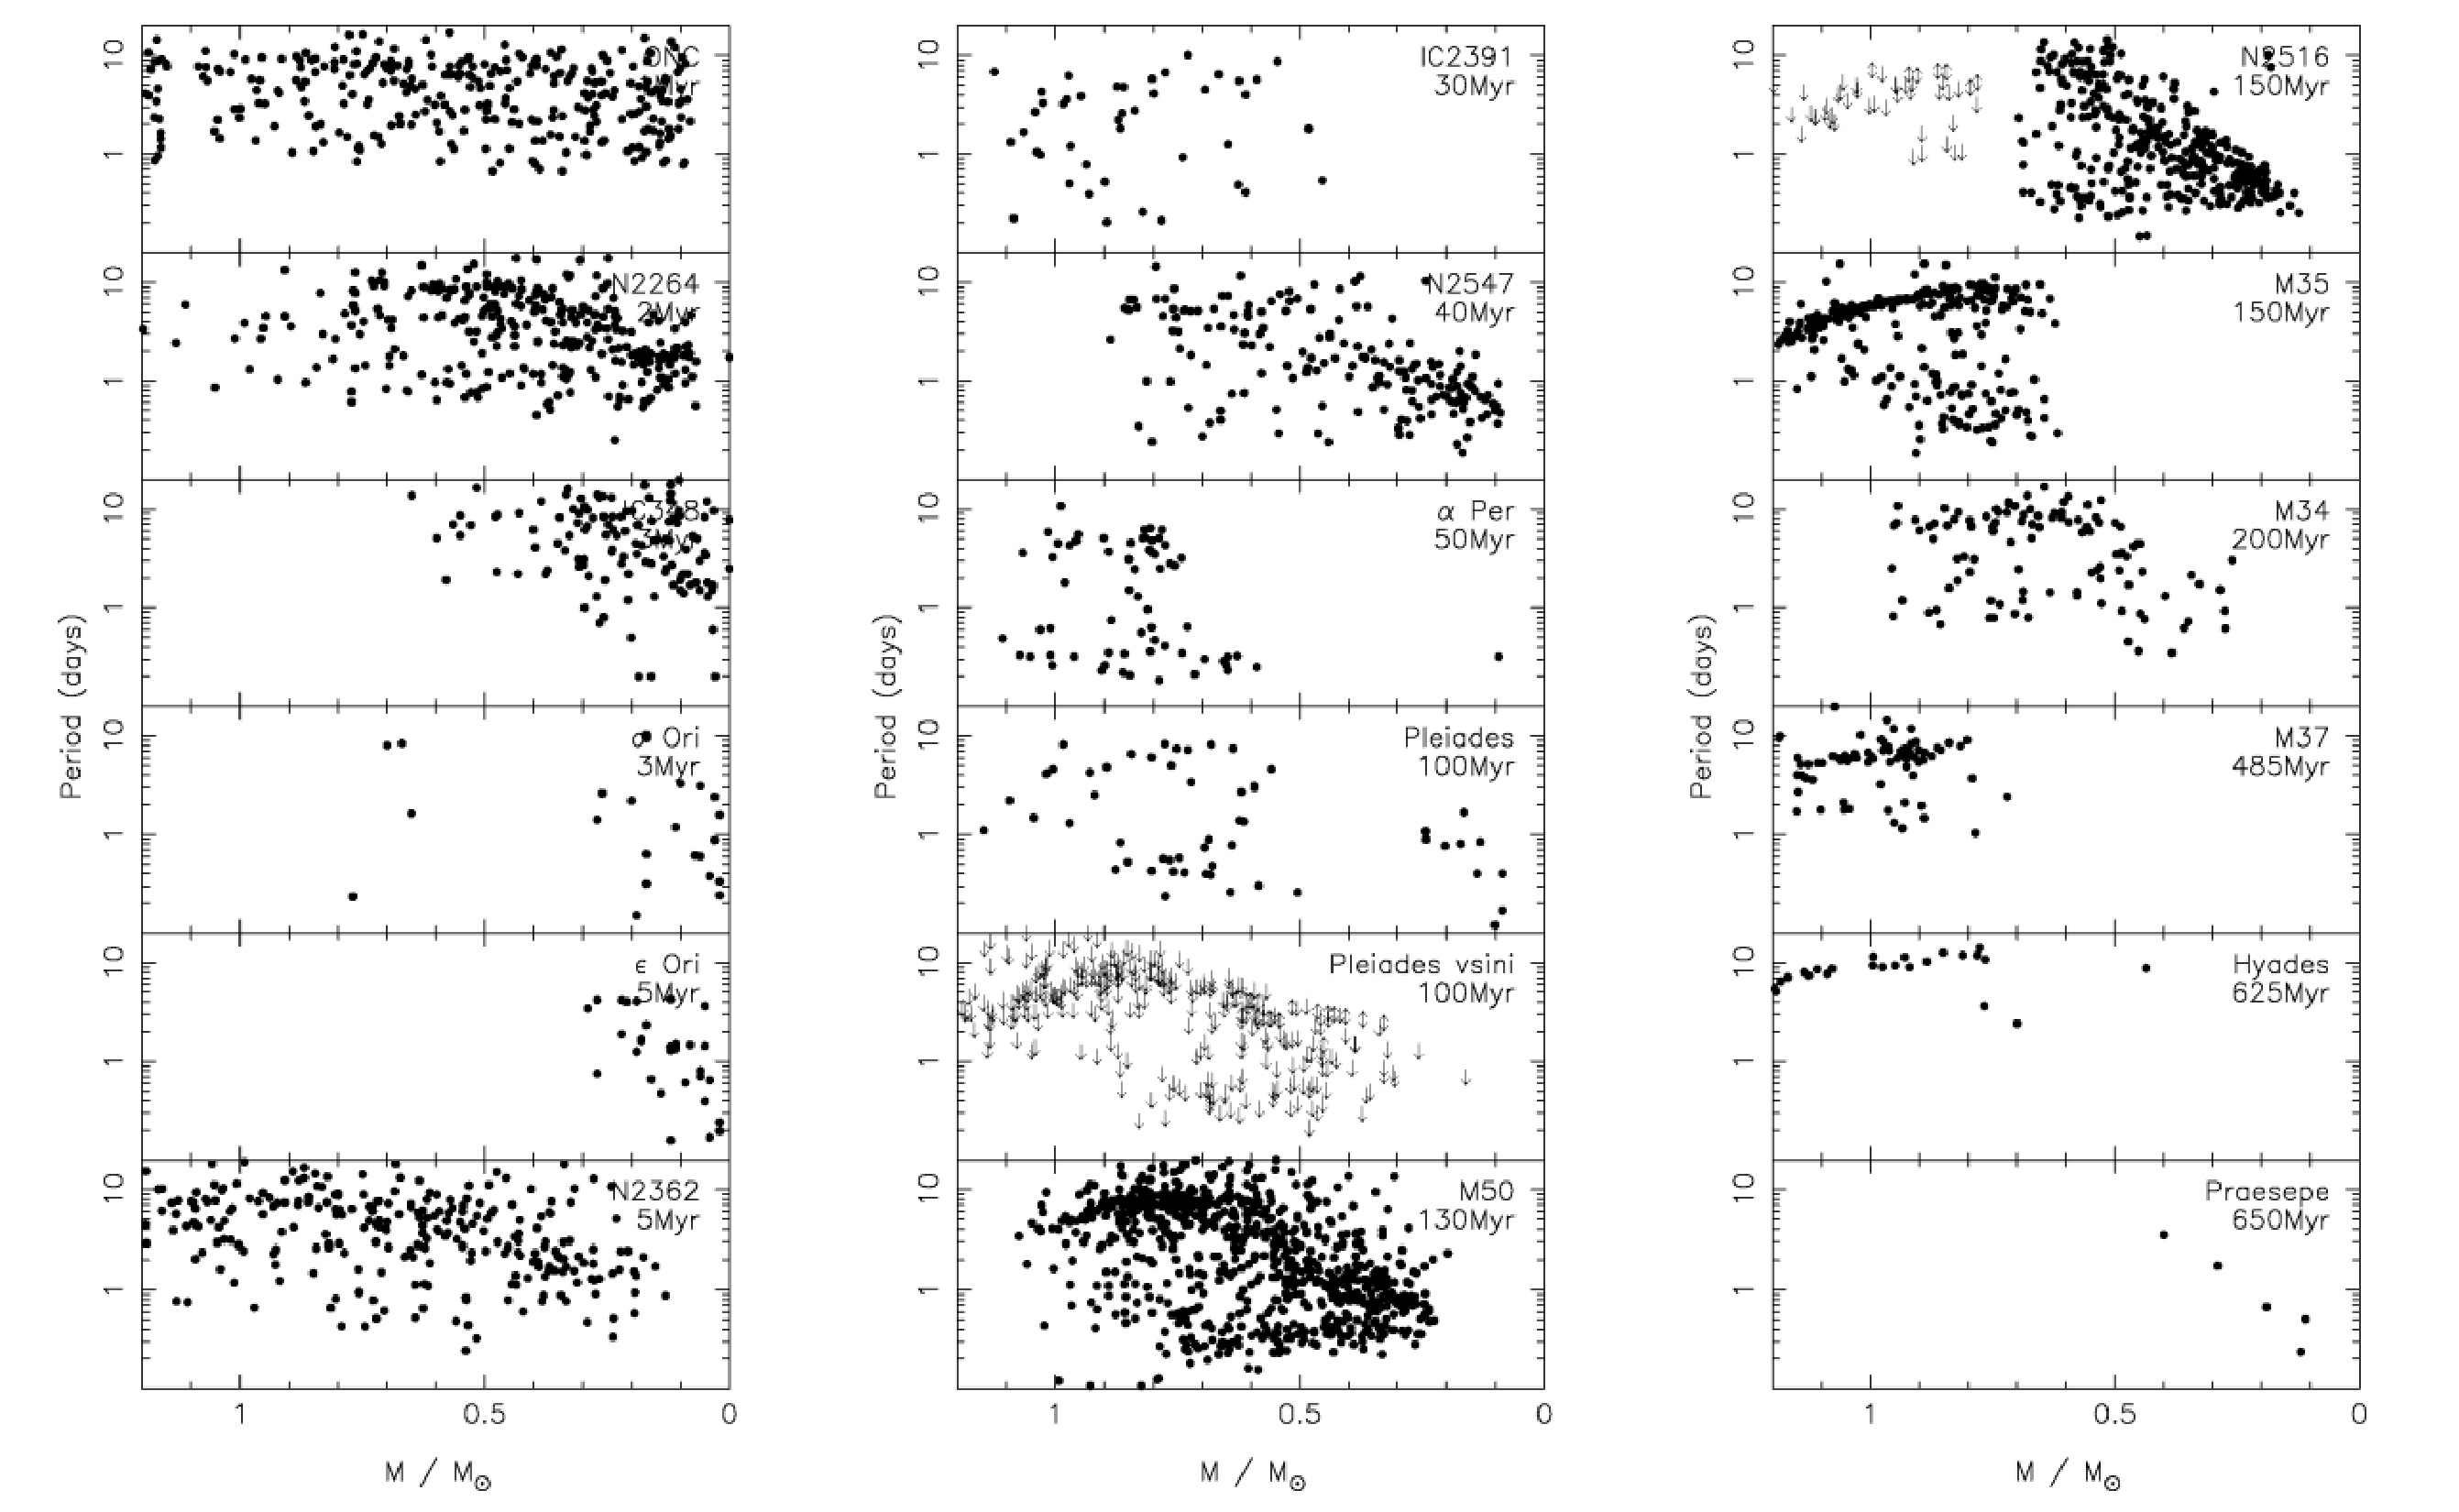
\includegraphics[width=6in, clip=true]{figures/irwin.pdf}
\caption{Figure from \citet{Irwin2009}. A compilation of most of the available
rotation periods for stars in open clusters with $M < 1.2 M_\odot$ in
2009.}
\label{fig:solar_spectrum}
\end{center}
\end{figure}

Gyrochronology, a term coined by \citet{Barnes2003}, is the inference of
stellar ages from rotation periods.
Many models for the prediction of the rotational evolution of stars have been
developed by different groups.
Some of these \citep[\eg][]{Vansaders, Reiners2012, Brown} use physical models
of rotating stars with magnetic fields, where the rate of angular momentum
loss is related to the rotation period and field strength, and evolve those
stars forward in time.
Although these models are based on the physical processes at play, they must
still be calibrated using observations since the models are over-simplistic.

An alternative approach is an entirely empirical one where simple functional
forms are fit to the observations \citep[\eg][]{Barnes2007, Mamajek2008,
Meibom2010}.
\citet{Barnes2003} proposed the following functional form for the relation
between period, colour and age, \begin{equation} \label{eq:Barnes2007_2} P =
A^n \times a(B-V-c)^b, \end{equation} where $P$ is rotation period (in days),
$A$ is age (in Myr), $B$ and $V$ are B and V band magnitudes respectively and
$a$, $b$, $c$ and $n$ are dimensionless free parameters.
\citet{Barnes2007} used rotation periods for stars in open clusters ranging in
age from 30-600 Myr to calibrate this relation.
This same functional form was used by \citet{Mamajek2008} and
\citet{Meibom2010} who also used young clusters to recalibrate the
gyrochronology model.

\section{Other age diagnostics}

\subsection{Activity}
Young stars are active because their rapid rotation drives the magnetic dynamo
in their convection zones \citep{Noyes1984}.
As their rotation periods decay, so does their activity.
Although stellar activity originates from one mechanism only: magnetism,
it manifests in a variety of detectable ways.
These are listed below.
\begin{itemize}
\item{Star spots.
Surface differential rotation, where the equator rotates at a different speed
to the poles (in the Sun it rotates faster), twists the magnetic flux into
tubes which emerge from the stellar surface.
The convection of material at the points where they emerge is inhibited and
these areas are cooler and darker as a result.
These cool, dark regions are called Sun spots on the Sun and star spots on the
surfaces of other stars.
Because these regions are darker, the integrated, optical flux emitted by a
star when there are more spots on the surface is decreased.
These decreases in brightness are detectable on the time scale of the stellar
rotation period, where spots rotate into and out of view, and on longer
timescales---the overall activity cycle.
The Sun has an activity cycle that lasts 11 years.
During periods of low activity the Solar surface has few star spots and this
number increases up to hundred of spots during the Solar maximum.}
\item{Chromospheric activity.
Magnetic activity in stellar chromospheres produces emission in the cores of
singly ionised calcium H (3969.5$\AA$) and K\footnote{The H and K letters
indicate the Fraunhofer designation. Fraunhofer assigned letters to the
absorption lines
he detected in the Solar spectrum.}
(3933.7$\AA$) lines.
This emission reversal is produced by the excitation of Ca$^+$ electrons to a
higher energy level via magnetic heating.
Just as with rotation period, chromospheric activity decreases with time.
Relations between age and chromospheric activity have, just as with rotation
period, been calibrated \citep[\eg][]{Soderblom1991, Donahue1993,
Lachaume1999, Mamajek2008}.
Chromospheric activity is usually quantified via the R$\prime_{HK}$ index,
defined as the flux excess in the lines, normalised to the bolometric flux.
The drawback of using chromospheric activity indices are similar to the
drawbacks of gyrochronology: the data are sparse and particularly so at late
ages and low masses.
Crucially though, measurements of Ca II H \& K emission are difficult to
obtain since high-resolution spectra are required.
}
\item{UV and X-ray flux.}
Magnetic heating excites photons to high energies, producing substantial UV
and X-ray fluxes.
Since M dwarfs have large convective zones, some even being fully convective,
they are highly active.
Their UV flux is significant which is currently causing ripples in the
exoplanet community.
M dwarfs with transiting exoplanets are premium targets for follow-up with the
James Webb Space Telescope (JWST) since their petite size relative to their
Earth-radius planets provides deep transits.
The large signal-to-noise ratios of these deep transits will allow JWST to
search for biomarkers in the atmospheres of these planets.
However, since M dwarfs are more active than G dwarfs, and their habitable
zones are closer in, any potential life on an Earth-twins may have been
obliterated by the extreme UV flux.
\item{Flare rate.
Convective turbulence in low-mass stars generates magnetic flux tubes.
Differential rotation then causes these flux tubes to twist around each other,
becoming entangled.
Magnetic reconnection causes the acceleration of particles and a huge amount
of energy is released into the Inter-Stellar Medium (ISM).
The flare rate is related to the mean flare energy via a power and both of
these properties are related to the strength of the stellar magnetic field.
Flares occur extremely often in M dwarfs, the most magnetically active stars,
with rates between ... and ....
% FIXME: how much energy is released?
% FIXME: what drives differential rotation?
}
\end{itemize}

\subsection{Lithium depletion boundary}
The Lithium Depletion Boundary (LDB) can be used as an age diagnostic for
young, low mass ($<1M_\odot$) stars.
As these young stars contract on the Pre-Main Sequence (PMS) their core
temperature increases.
When it reaches $\sim2.5\times10^6$ K, lithium is destroyed via $^7$Li$(p,
\alpha)^4$He and $^6$Li$(p, \alpha)^3$He proton capture reactions
\citep[\eg][]{Bodenheimer1965}.
The time taken for a star to reach these temperatures depends on their mass.
The lowest mass PMS stars are fully convective, so the mixing timescale is
very short and lithium depletion takes place very rapidly.
For young stellar groups therefore, the mass at which the LDB (the boundary
stars that do and do not show lithium in their atmospheres) is located is a
very sensitive function of age \citep{Basri1996}.
LDB dating can be very precise \citep{Burke2004}, however it is only
applicable to young groups of stars (20 Myr < age < 200 Myr) since by this
time Lithium has disappeared from the atmospheres of all members, regardless
of their mass.

\subsection{Dynamics}
Stellar populations in the Milky Way galaxy can be localised into four groups:
the bulge, the thin disk, the thick disc and the halo.
Each of these stellar populations has a different distribution of stellar
ages.
The bulge is comprised of old stars.
It is characteristically red because the only remaining stars on the MS are
low-mass.
The thin disk is comprised of young stars.
This is the main star-forming part of the galaxy as the spiral arms, density
waves of molecular gas that readily collapses into protostars, reside in the
thin disk.
The orbits of thin disk stars get heated over time.
Close encounters with neighbouring stars boost their orbital energies and many
thin disc stars find themselves `kicked' out of the galactic plane into the
`thick disc'.
The thick disc is statistically older than the thin disc since the majority of
its residents have had time to experience one or more close encounters.
The halo is even older still: these stars have been displaced even further
from the thin disk in which they were born.
Since the probability of experiencing a close encounter increases with time,
stars with higher proper motions are likely to be older.
However, although a rapidly moving star is likely to be older than a slowly
moving star, stellar-orbit heating is a stochastic process and therefore
cannot always be relied upon.

\section{Probabilistic Statistical methods}

A core part of this thesis is the statistical methods that are employed.
None of the methods used here are new in themselves, but many have not been
previously used on the sorts of problems that are presented here or in an
astronomical context.
I will now discuss them in the order in which they feature in the subsequent
chapters of this thesis.

\subsection{Multi-dimensional and unknown uncertainties: hierarchical
probabilistic modelling}
In some cases in astronomy, the only significant uncertainties are on
the dependent variable.
This is often the case with time-series or spectra and assuming that the
independent variable uncertainties are negligible is a reasonable assumption.
In a case where one wants to fit a model to data where the only significant
uncertainties lie in the $y$ direction, those uncertainties are Gaussian, the
measurements are independent and there is no correlated noise, it may be
appropriate to use the Gaussian likelihood function.
For example the likelihood of $y$-values, given some $x$-values, some model
parameters, $\mathbf{\theta}$ and some $y$-direction uncertainties, $\sigma$,
the likelihood can be written
\begin{equation}
    p(y|x, \sigma, \mathbf{\theta}) = \prod_{i=1}^N
    \frac{1}{\sqrt{2\pi\sigma_i^2}}
    \exp\left(-\frac{[y_i - \mu(x_i, \mathbf{\theta})]^2}{2\sigma_i^2}\right),
\end{equation}
where $\mu$ is the mean model.
It is often more practical to use the logarithm of this function,
\begin{equation}
    \ln\mathcal{L} =
    -\frac{1}{2} \sum_{i=1}^N \left[\frac{[y_i - \mu(x_i,
    \mathbf{\theta})]^2}{\sigma_i^2} +
    \ln\left(2\pi\sigma_i^2\right) \right],
\end{equation}
\label{eq:lnlike}
which is also known as $-\frac{1}{2}\chi^2$.

In many fitting-model-to-data problems in the astronomical literature,
a frequentist approach is taken and $\chi^2$ is minimised (which is the
equivalent of maximising the log-likelihood).
The probabilistic (Bayesian) approach however is to multiply this likelihood
by a prior to produce a posterior Probability Density Function (PDF).
\begin{equation}
Bayes rule
\end{equation}
The prior represents one's prior beliefs about the model parameters,
$\mathbf{\theta}$.
There is a wide range of literature available on the science behind choosing
priors which is beyond the scope of this thesis.
% CITATIONS

Returning to equation \ref{eq:lnlike}, it is trivial to modify this function
for the case where the $y$-direction uncertainties are unknown, or
under-(or over)-estimated.
In this case one could write
\begin{equation}
    \ln\mathcal{L} =
    -\frac{1}{2} \sum_{i=1}^N \left[\frac{[y_i - \mu(x_i,
    \mathbf{\theta})]^2}{\sigma_i^2 + s^2} +
    \ln\left(2\pi(\sigma_i^2 + s^2\right) \right],
\end{equation}
where $s^2$ is the additional variance needed to explain the scatter in the
data.

In chapter \ref{chapter:flicker} a modification to the above equation is used
to fit a line to data where the uncertainties are underestimated.
This is a hierarchical problem, since there are two parameters that describe
the model (a straight line), $\alpha$ and $\beta$, where $\mu = \alpha +
\beta x$ and a parameter describes the standard deviation of a Gaussian
spanning the mean model.
In other words, the `true' value of variable $y$---the value that would have
been measured if there were no observational uncertainties, $\bar{y}$ is drawn
from a Gaussian with mean, $\mu = \alpha + \beta \bar{x}$ and standard
deviation, $s$:
\begin{equation}
\bar{y} \sim \mathcal{N}(\alpha + \beta\bar{x}, s^2),
\end{equation}
and the {\it observations}, $y_{obs}$ are in turn drawn from Gaussians with
$\mu = \bar{y}$ and standard deviations described by the individual
observational uncertainties, $\sigma_{obs}$:
\begin{equation}
y_{obs} \sim \mathcal{N}(\bar{y}, \sigma_{obs}^2).
\end{equation}
Since it is the observations that are modelled, not the latent parameter,
$\bar{y}$, this is a hierarchical process.

Equation \ref{eq:lnlike} can also be modified for the simple case of fitting a
straight line to data, where the $y$-direction observational uncertainties are
unknown {\it and} the $x$-direction uncertainties are non-negligible.
Starting from equations 26, 29, 31 and 32 of \citet{Hogg2010},
$\mathbf{S_i}$ is the covariance tensor,
\begin{eqnarray}
    \mathbf{S_i} &\equiv& \left( \begin{array}{cc}
                    \sigma_{x}^2 & \sigma_{x,y} \\
                    \sigma_{x,y} & \sigma_{y}^2
\end{array}\right),
\end{eqnarray}
\label{eq:covariance_tensor}
$\mathbf{\hat{\nu}}$ is a unit vector orthogonal to the line with slope
$\alpha$,
\begin{equation}
    \mathbf{\hat{\nu}} = \frac{1}{\sqrt{1 + \alpha^2}} \left( \begin{array}{c}
                                                    -\alpha \\
                                                    1
    \end{array}\right),
\end{equation}
\label{eq:unit_vector}
the variance is given by,
\begin{equation}
    \Sigma_i^2 = \mathbf{\hat{\nu}}^T \mathbf{S_i} \mathbf{\hat{\nu}}
\end{equation}
\label{eq:variance}
and the log-likelihood can be written,
\begin{equation}
    \ln\mathcal{L} = - \frac{1}{2} \sum_{i=1}^N \left[
    \frac{\Delta_i^2}{\Sigma_i^2} + \ln|\mathbf{S_i}| \right].
\end{equation}
\label{eq:ndlnlike}
By modifying equation \ref{eq:covariance_tensor} to be
\begin{eqnarray}
    \mathbf{S_i} &=& \left( \begin{array}{cc}
                    \sigma_{x}^2 & 0 \\
                    0 & \sigma_{y}^2 + s^2
\end{array}\right),
\end{eqnarray}
\label{eq:covariance_tensor_mod}
since we assume that the covariance between $x$ and $y$ is negligible,
substituting \ref{eq:covariance_tensor_mod}, \ref{eq:unit_vector} \&
\ref{eq:variance} into \ref{eq:ndlnlike} gives
\begin{equation}
    \ln(\mathcal{L}) = -\frac{1}{2} \sum_{i=1}^N
    \left( \frac{\left[ y_i - (\alpha + \beta x_i) \right]^2}
    {\beta^2\sigma_{x, i} + \sigma_{y, i}^2 + s^2} + \ln[\sigma_{x,
    i}^2(\sigma_{y, i}^2 + s^2)]
    \right)
\end{equation}.
This is the equation used in chapter \ref{chapter:flicker} to perform such an
analysis with astrophysical data.

In cases with more complicated mean models, it is not so easy to arrive at an
analytic solution.
For example, a similar problem is approached in chapter \ref{chapter:gyro}.
Here, the extra variance parameter, $s$ is not used (although it should be
included in future analyses!), however the uncertainties in the $x$, $y$, and
this time $z$ too, directions are large.
The model is not a simple two-dimensional line as in the above case, it is the
three-dimensional gyrochronology equation \ref{eq:barnes} where $y$ is
rotation period, $x$ is age and $z$ is B-V colour.
In this case, an approximation must be made in order to take the uncertainties
on all dimensions into account.
This approximation is made via sampling and is described in chapter
\ref{chapter:gyro}.

\subsection{Methods for removing systematics}
\label{sec:detrending}

`Detrending' is a word that has been adopted by astronomers to mean removing
systematic trends caused by non-physical (\eg instrumental) variations in the
experiment conditions.
This process can be applied to any data set that contains correlated noise, be
it a time series, image or spectrum, however `detrending' usually pertains
specifically to time series analysis, and light curves in particular.
The detrending process involves the generation of some model of the systematic
features that can be generated and then subtracted from the light curve.
This implies that the contribution of systematics to the light curve are known
{\it a priori}.
Of course in reality, the contributions coming from the signal and the noise
can never be known completely, so must be approximated.
In some cases this approximation is close to the truth, or doesn't need to be
for the purposes of extracting science from the data (for example, if
instrumental systematics exist on very different timescales to the signal of
interest).
However, in many cases the noise model cannot be adequately approximated.
At best this leads to inaccurate inferences about the physical system being
studied and at worse it leads to false positive detections and false negative
non-detections.

In \textsection \ref{chapter:sip} I present a method for extracting periodic
signals from \ktwo\ light curves, without detrending.
In what follows I review a selection of detrending methods.

\subsection{Rotation period inference}

\subsubsection{ACF}
An AutoCorrelation Function (ACF) was first used to measure rotation periods
by \citet{Mcquillan2013} who developed the method specifically for \kepler\
data.

\subsubsection{Lomb-Scargle}
\subsubsection{Wavelets}
\subsubsection{Spectroscopy}
